\section{Benchmark 2: Magnetic Field Analogy of Vortex Rings}

To validate the Vortex Æther Model (VAM) correspondence between vortex-induced swirl and classical electromagnetism, we compute the velocity field of a circular vortex ring and compare it with the magnetic dipole field generated by a current loop.

\subsection{Biot–Savart Field from a Vortex Ring}

Using the Biot–Savart law for thin-core vortex filaments, the velocity field in the $x$–$z$ plane is computed for a toroidal ring of circulation $\Gamma$:

\begin{equation}
\vec{v}(\vec{x}) = \frac{\Gamma}{4\pi} \oint \frac{(\vec{dl} \times \vec{r})}{|\vec{r}|^3} \, d\ell
\end{equation}

\noindent
The resulting flow field exhibits closed toroidal symmetry, identical in structure to the magnetic field surrounding a circular current-carrying wire.

\begin{figure}[H]
    \centering
    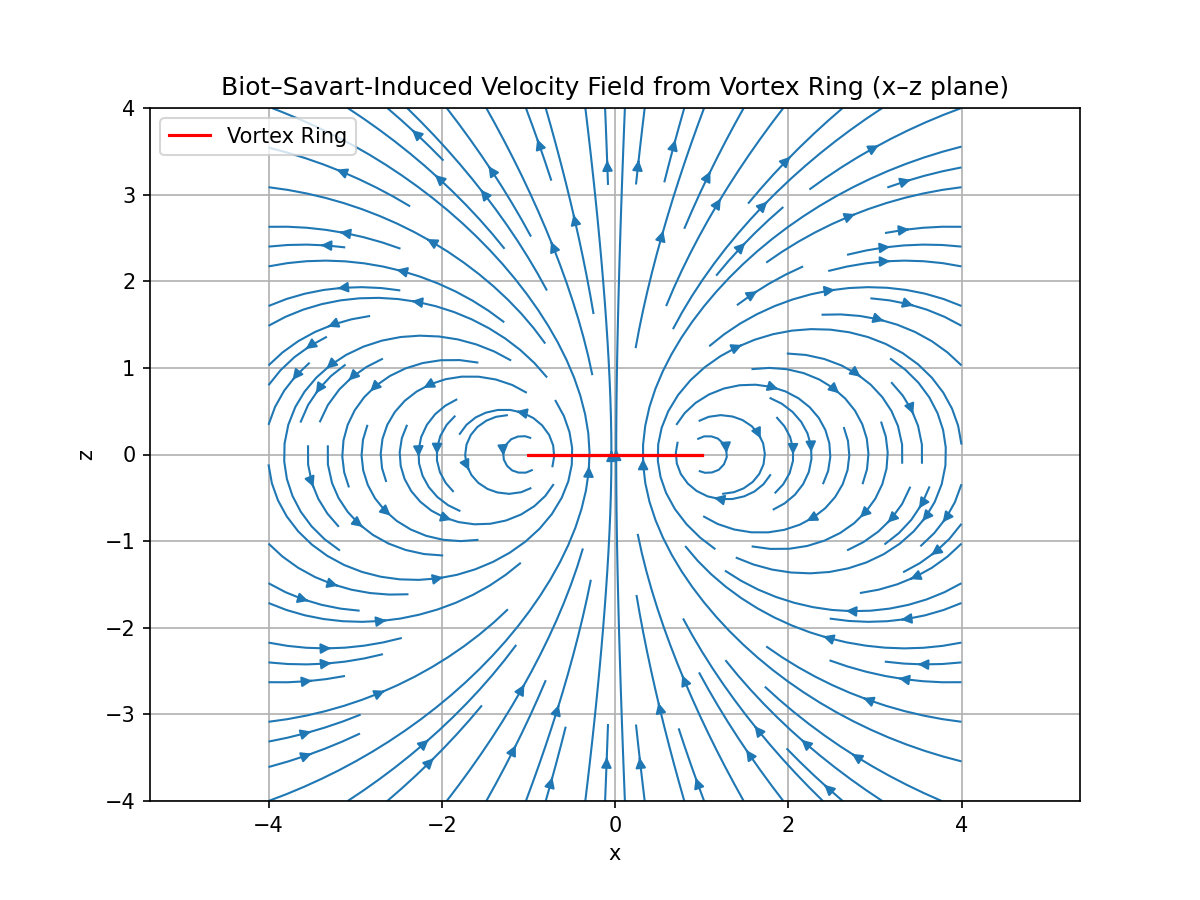
\includegraphics[width=0.6\textwidth]{images/dipole_1}
    \caption{Velocity field induced by a vortex ring (Biot–Savart integration in the $x$–$z$ plane). The flow loops around the ring, mimicking magnetic dipole field lines.}
\end{figure}

\subsection{Comparison with Magnetic Dipole Field}

For comparison, the theoretical magnetic dipole field is computed using:

\begin{equation}
\vec{B}(\vec{r}) = \frac{\mu_0}{4\pi} \left[ \frac{3\vec{r}(\vec{m} \cdot \vec{r}) - r^2 \vec{m}}{r^5} \right]
\end{equation}

\noindent
where $\vec{m}$ is the dipole moment aligned along the $z$-axis. The normalized field lines are shown below:

\begin{figure}[H]
    \centering
    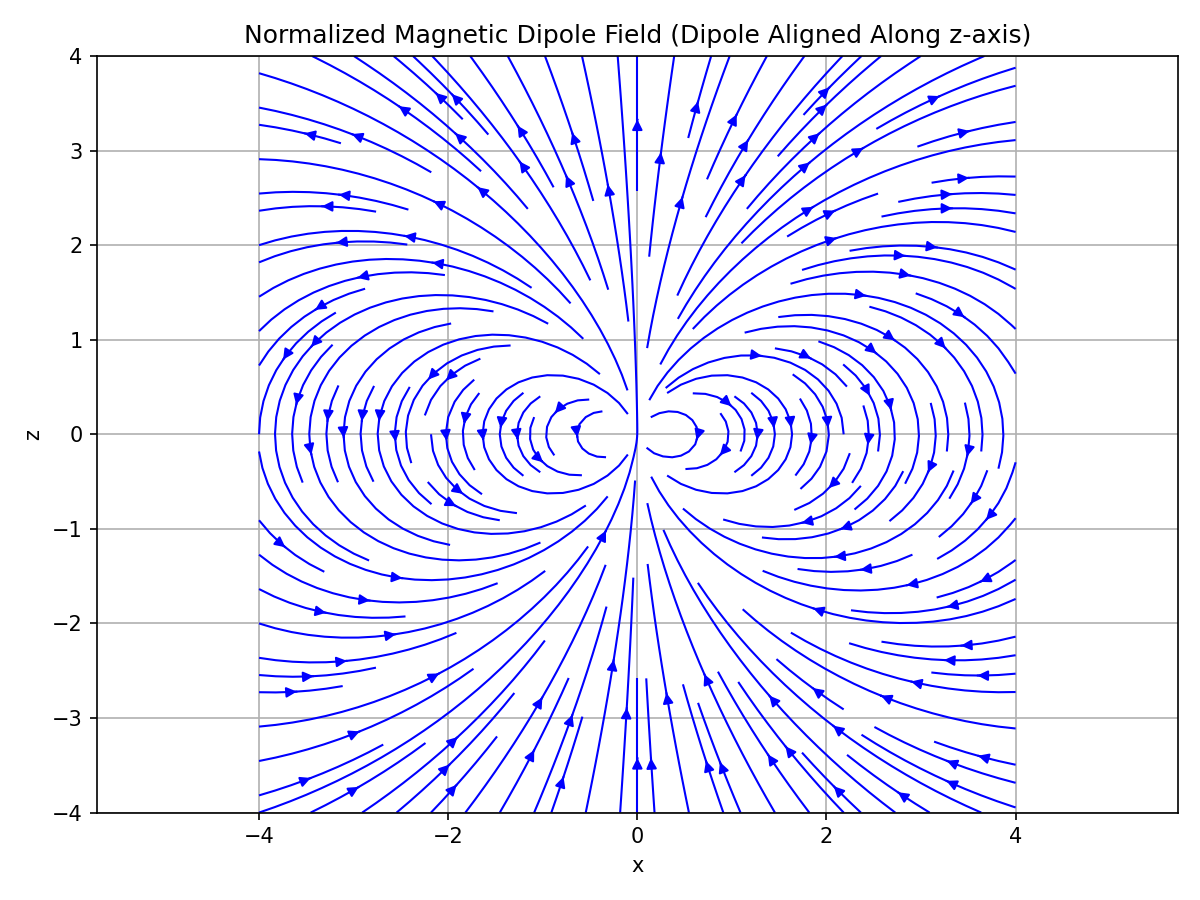
\includegraphics[width=0.6\textwidth]{images/dipole_2}
    \caption{Normalized magnetic dipole field aligned along the $z$-axis. The structure is qualitatively identical to the vortex ring field, confirming the VAM–EM mapping.}
\end{figure}

\subsection{Vorticity and Helicity Structure}

In the VAM formulation, the vorticity field is defined as the curl of the velocity field:

\begin{equation}
\vec{\omega} = \nabla \times \vec{v}
\end{equation}

In the $x$–$z$ plane, the dominant component of vorticity is typically the $y$-component:

\begin{equation}
\omega_y = (\nabla \times \vec{v})_y = \frac{\partial v_z}{\partial x} - \frac{\partial v_x}{\partial z}
\end{equation}

This component represents the out-of-plane swirl associated with the toroidal structure of the vortex ring.

\begin{figure}[H]
    \centering
    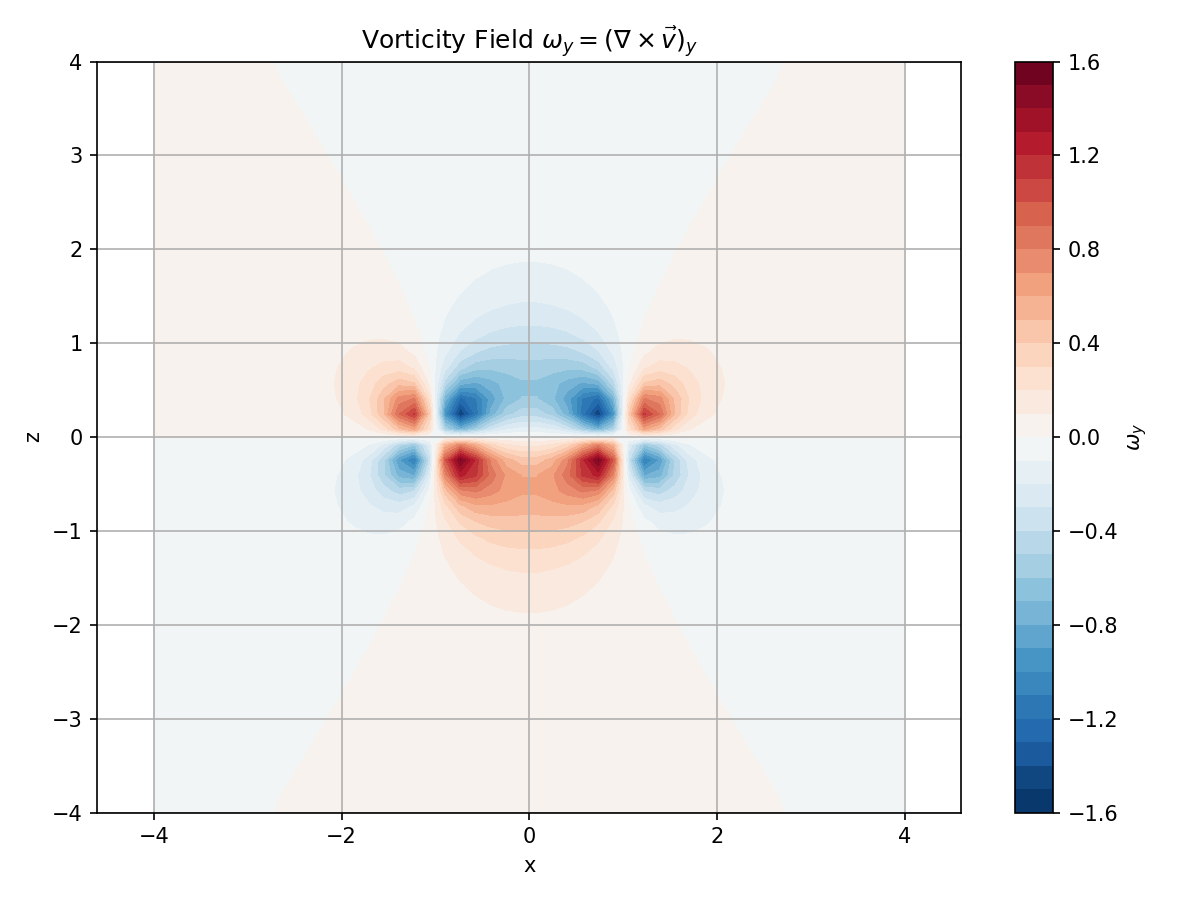
\includegraphics[width=0.6\textwidth]{images/dipole_3}
    \caption{Vorticity field $\omega_y = (\nabla \times \vec{v})_y$ in the $x$–$z$ plane. The field is concentrated around the vortex core and exhibits the expected ring-like symmetry.}
\end{figure}

To measure the alignment between the velocity and vorticity vectors — i.e., the degree of local swirl coherence — we compute the helicity density:

\begin{equation}
h(\vec{x}) = \vec{v}(\vec{x}) \cdot \vec{\omega}(\vec{x})
\end{equation}

Regions of nonzero helicity density indicate topological twisting, which in VAM correlates directly with physical properties such as electric charge and spin polarization.

\begin{figure}[H]
    \centering
    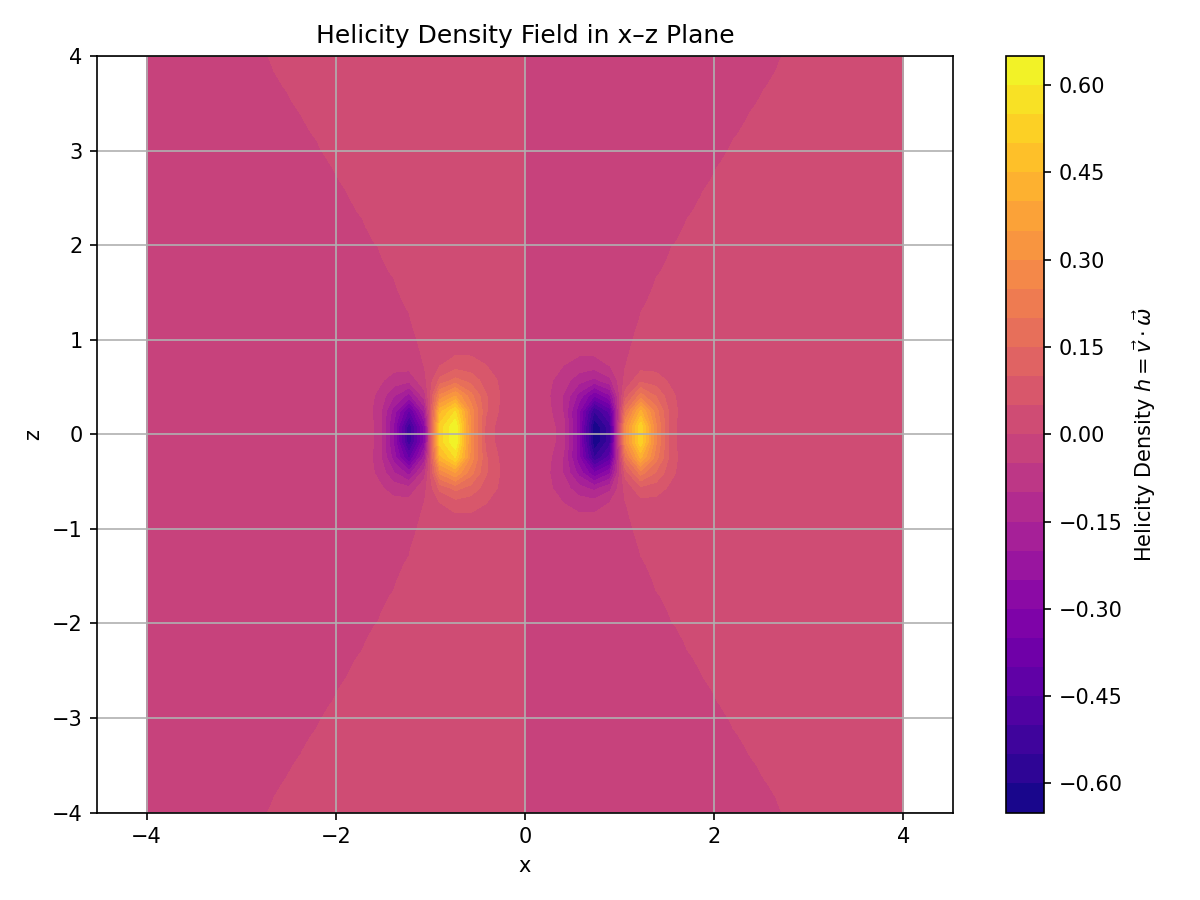
\includegraphics[width=0.6\textwidth]{images/dipole_4}
    \caption{Helicity density $h = \vec{v} \cdot \vec{\omega}$ in the $x$–$z$ plane. Areas with high helicity indicate topologically charged or chiral vortex behavior, as seen in photon-like toroidal configurations.}
\end{figure}


\subsection{Conclusion}

This benchmark confirms that the velocity field induced by a vortex ring in an ideal fluid reproduces the same topological structure as a magnetic dipole field in classical electromagnetism. In VAM, the magnetic field is interpreted as the curl of the local æther velocity field: $\vec{B} \sim \nabla \times \vec{v}$.

